%!TEX root = edance.tex
%%%%%%%%%%%%%%%%
%  CHAPTER 12  %
%%%%%%%%%%%%%%%%
\chapter{Single-Stage Amplifiers}
\graphicspath{{./figs_amps_single_stage/}}
%%%%%%%%%%%%%%%%%%%%%%%%%%%%%%%%%%%%%%%%%%%%%%%%%%%%%%%%%%%%%%%%%%%%%%%%%%%%%%%%%%%%%%%%
%%%%%%%%%%%%%%%%%%%%%%%%%%%%%%%%%%%%%%%%%%%%%%%%%%%%%%%%%%%%%%%%%%%%%%%%%%%%%%%%%%%%%%%%
%                                   SECTION 12.1                                       %
%%%%%%%%%%%%%%%%%%%%%%%%%%%%%%%%%%%%%%%%%%%%%%%%%%%%%%%%%%%%%%%%%%%%%%%%%%%%%%%%%%%%%%%%
%%%%%%%%%%%%%%%%%%%%%%%%%%%%%%%%%%%%%%%%%%%%%%%%%%%%%%%%%%%%%%%%%%%%%%%%%%%%%%%%%%%%%%%%
\section{Chapter Preview}
This chapter reviews the three important single-stage amplifier topologies.  Understanding these single-stage amplifiers is crucial, as we will build on these amplifiers in the following chapters to build more complex and higher performance multi-stage amplifiers.  Intimate knowledge of the input and output impedance and the voltage/current gains is needed in order to move onto more complex amplifiers.  We will therefore begin by reviewing the fundamentals of amplifiers using two-port models, and then we will show how each single-stage amplifier can be classified accordingly.  
%%%%%%%%%%%%%%%%%%%%%%%%%%%%%%%%%%%%%%%%%%%%%%%%%%%%%%%%%%%%%%%%%%%%%%%%%%%%%%%%%%%%%%%%
%%%%%%%%%%%%%%%%%%%%%%%%%%%%%%%%%%%%%%%%%%%%%%%%%%%%%%%%%%%%%%%%%%%%%%%%%%%%%%%%%%%%%%%%
%                                   SECTION 12.2                                       %
%%%%%%%%%%%%%%%%%%%%%%%%%%%%%%%%%%%%%%%%%%%%%%%%%%%%%%%%%%%%%%%%%%%%%%%%%%%%%%%%%%%%%%%%
%%%%%%%%%%%%%%%%%%%%%%%%%%%%%%%%%%%%%%%%%%%%%%%%%%%%%%%%%%%%%%%%%%%%%%%%%%%%%%%%%%%%%%%%
\section{Review Two-Port Amplifiers}
%%%%%%%%%%%%%%%%%%%%%%%%%%%%%%%%%%%%%%%%%%%%
%             SUBSECTION 12.2.1            %
%%%%%%%%%%%%%%%%%%%%%%%%%%%%%%%%%%%%%%%%%%%%
\subsection{One-Port Equivalent Models}
%%%%%%%%%%%%%%%%%%%%%%%%%%%%%%%%%%%%%%%%%%%%
%                 FIGURE                   %
%%%%%%%%%%%%%%%%%%%%%%%%%%%%%%%%%%%%%%%%%%%%
\begin{figure}[tb]
\begin{center}
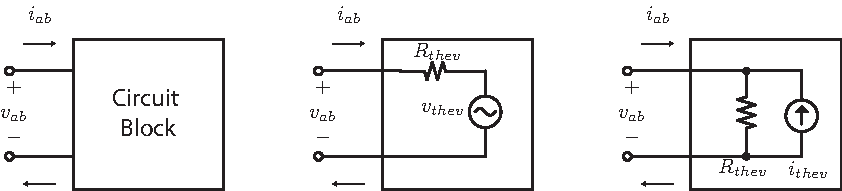
\includegraphics[scale=1]{oneports}
\end{center}
\caption{A blackbox one-port linear circuit can be represented as a Thevenin or Norton equivalent.} \label{fig:oneports}
\end{figure}

Consider any linear circuit as a blackbox with a pair of exposed terminals.  We know from basic circuit theory that we can represent this blackbox as an equivalent Thevenin or Norton model (Fig.~\ref{fig:oneports}).  This is also true of amplifiers, but amplifiers have two important differences.  First, most amplifiers have an input and an output port, where a ``port" is a  pair of terminals.  Often one terminal is shared, or ``common", between the ports, such as the ground connection.   The other important difference is that two-port amplifiers do not have any sources (of the independent variety) in them.  Finally, we assume that an amplifier is a \textit{unilateral} block, meaning the output depends on input but input is independent of output.  In other words, signals travel in one direction, but not the other.  This is why the schematic symbol for an amplifier is often drawn as a triangle (think of an arrow).  In general, though, the output port depends linearly on the current and voltage at the input and output ports, because there's output impedance.  

Why are amplifiers unilateral?  Think about the small-signal model of a FET or BJT.  The output depends on the input $v_{\pi}$ or $v_{gs}$ through $g_m$ but the input is more or less independent of the output, except for the effects of the small ``overlap" or junction capacitance $C_{gd}$/$C_\mu$.  As long as the ``forward" gain $g_m$ is much larger than the reverse, $j\omega C_{gd}$, then the amplifier is unilateral.  At low frequencies, this is certainly true and a useful simplifying approximation.
%%%%%%%%%%%%%%%%%%%%%%%%%%%%%%%%%%%%%%%%%%%%
%             SUBSECTION 12.2.2            %
%%%%%%%%%%%%%%%%%%%%%%%%%%%%%%%%%%%%%%%%%%%%
\subsection{Small-Signal Two-Port Models}
%%%%%%%%%%%%%%%%%%%%%%%%%%%%%%%%%%%%%%%%%%%%
%                 FIGURE                   %
%%%%%%%%%%%%%%%%%%%%%%%%%%%%%%%%%%%%%%%%%%%%
\begin{figure}[tb]
\begin{center}
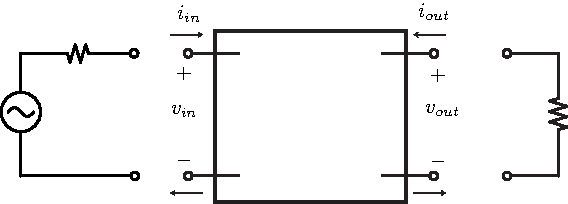
\includegraphics[scale=1]{2port_ss}
\end{center}
\caption{Similar to a one-port, a two-port linear circuit can be represented using an equivalent model.  If the blackbox is an amplifier, we can choose among many different representations shown in Fig.~\ref{fig:vi_amp} and Fig.~\ref{fig:gm_z_amp}.}
\label{fig:2port_ss}
\end{figure}
 
A linear two-port box, shown in Fig.~\ref{fig:2port_ss}, under the unilateral assumption, can be represented as a generic amplifier in four different ways, as shown in Fig.~\ref{fig:vi_amp} and Fig.~\ref{fig:gmamp}.  Note that signals can be represented as voltage, or as current, or some combination of the two.  Also it's important to note that any real amplifier has input impedance $R_{in}$ and output impedance $R_{out}$ because both voltages and currents (power) are needed for the circuit to work.  
%%%%%%%%%%%%%%%%%%%%%%%%%%%%%%%%%%%%%%%%%%%%
%              SUB-SUBSECTION              %
%%%%%%%%%%%%%%%%%%%%%%%%%%%%%%%%%%%%%%%%%%%%
\subsubsection{Two-Port Small-Signal Voltage Amplifier}
Let's begin with Fig.~\ref{fig:vi_amp}a, or a Voltage Amplifier.  This is perhaps the most straightforward amplifier to understand, as both input/output signals are voltages.  Recall that an ideal voltage amplifier has a very large input impedance $R_{in}$ so that it does not ``load" the driver circuitry, and so most of the applied voltage appears across $R_{in}$ rather than the source impedance.  Likewise, for similar reasons, the voltage amplifier should have a very small output impedance $R_{out}$.
%%%%%%%%%%%%%%%%%%%%%%%%%%%%%%%%%%%%%%%%%%%%
%                 FIGURE                   %
%%%%%%%%%%%%%%%%%%%%%%%%%%%%%%%%%%%%%%%%%%%%
\begin{figure}[tb]
\begin{center}
\begin{tabular}{c}
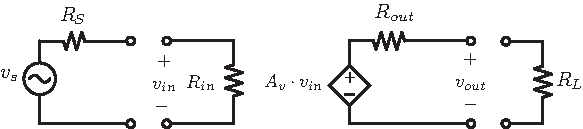
\includegraphics[width=.7\columnwidth]{vamp_label} \\
(a) \\
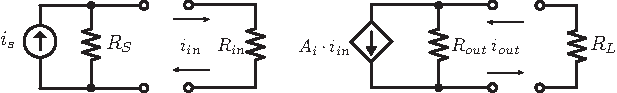
\includegraphics[width=.7\columnwidth]{iamp} \\
(b) \\
\end{tabular}
\end{center}
\caption{(a) A two-port voltage amplifier has internal gain $A_v$, input impedance $R_{in}$, and output impedance $R_{out}$.  (b) A two-port current amplifier has internal gain $A_i$, input impedance $R_{in}$, and output impedance $R_{out}$.}
\label{fig:vi_amp}
\end{figure}
%%%%%%%%%%%%%%%%%%%%%%%%%%%%%%%%%%%%%%%%%%%%
%              SUB-SUBSECTION              %
%%%%%%%%%%%%%%%%%%%%%%%%%%%%%%%%%%%%%%%%%%%%
\subsubsection{Two-Port Small-Signal Current Amplifier}
The dual of a Voltage Amplifier is the Current Amplifier, shown in Fig.~\ref{fig:vi_amp}.  The role of voltage and current are interchanged, and an input current into the amplifier is amplified and divided between the load and the internal output impedance $R_{out}$.  For this reason, we would like a current amplifier to have as large of an output impedance $R_{out}$ as possible, to maximize the current gain.  Also, a current amplifier with a low input impedance can ``steal" all the current from a source since a current divider favors the path of highest conductance.
%%%%%%%%%%%%%%%%%%%%%%%%%%%%%%%%%%%%%%%%%%%%
%              SUB-SUBSECTION              %
%%%%%%%%%%%%%%%%%%%%%%%%%%%%%%%%%%%%%%%%%%%%
\subsubsection{Two-Port Small-Signal Transconductance Amplifier}
%%%%%%%%%%%%%%%%%%%%%%%%%%%%%%%%%%%%%%%%%%%%
%                 FIGURE                   %
%%%%%%%%%%%%%%%%%%%%%%%%%%%%%%%%%%%%%%%%%%%%
\begin{figure}[tb]
\begin{center}
\begin{tabular}{c}
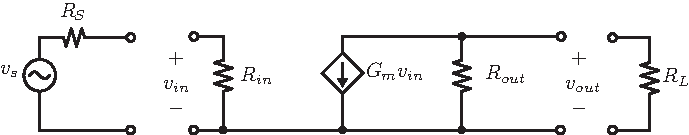
\includegraphics[width=.7\columnwidth]{gmamp} \\
(a) \\
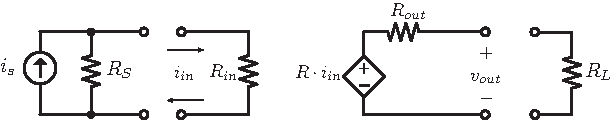
\includegraphics[width=.7\columnwidth]{ramp} \\
(b) \\
\end{tabular}
\end{center}
\caption{(a) A two-port transconductance amplifier has internal gain $G_m$, input impedance $R_{in}$, and output impedance $R_{out}$.  (b) A two-port trans-resistance amplifier has internal gain $R$, input impedance $R_{in}$, and output impedance $R_{out}$.}
\label{fig:gm_z_amp}
\end{figure}

The Transconductance Amplifier shown in Fig.~\ref{fig:gm_z_amp}a takes an input voltage and generates an output current, just like a conductor, but the signals are at different ports, making it a ``trans" conductor, effectively \emph{transporting} the signal from the voltage domain to the current domain.  Take a moment to consider that the concept of voltage and current domain only make sense with respect to the source and load impedance.  A good voltage source has low impedance with respect to the load, and a good current source has a high output impedance with respect to the load.  So a transconductance amplifier is effective if it presents a input high impedance, ideally infinite, and generates an output current with high output impedance.  A MOS transistor biased in saturation (and a BJT biased in the forward-active region) is almost an ideal transconductor, because its input is a high impedance at low frequencies, and its output is nearly open, due to the large output impedance of a transistor in saturation.  

Notice that the most general transconductance model has 4 separate terminals, but we've drawn a version with a common node, similar to the transistor hybrid-pi model. 
%%%%%%%%%%%%%%%%%%%%%%%%%%%%%%%%%%%%%%%%%%%%
%              SUB-SUBSECTION              %
%%%%%%%%%%%%%%%%%%%%%%%%%%%%%%%%%%%%%%%%%%%%
\subsubsection{Two-Port Small-Signal Trans-Resistance Amplifier}
The Trans-resistance amplifier is an amplifier that converts an input current into a voltage, as shown in Fig.~\ref{fig:gm_z_amp}b.  It's the dual of the Transconductance Amplifier, and ideally present a low input impedance at the input and drives the output with a low impedance voltage.  Trans-resistance amplifiers are also known as Trans-Impedance Amplifiers (TIAs) and play an important role in fiber optic communication, where the input light signal is a current (proportional to photon flux) that is converted to a voltage by a TIA.  Also, many sensors naturally generate a current signal (they have high source impedance) and need to be converted into voltage signals to drive other circuitry, such as Analog-to-Digital Converters (ADCs), which expect to be driven by a relatively low source impedance.  
%%%%%%%%%%%%%%%%%%%%%%%%%%%%%%%%%%%%%%%%%%%%
%             SUBSECTION 12.2.3            %
%%%%%%%%%%%%%%%%%%%%%%%%%%%%%%%%%%%%%%%%%%%%
\subsection{Input Impedance $Z_{in}$}
To calculate the input and output impedances of two-ports, we can simply use a test source at the input or output  in order to determine the equivalent load at each port, as shown schematically in Fig.~\ref{fig:2port_zin_vx}.  In a truly unilateral two-port, when probing the input port, the output port would play no role in determining the input impedance, and it could be left open-circuit, short-circuited, or terminated in an arbitrary impedance $Z$.  But in practice, circuits are not perfectly unilateral, and so we should have a convention for what to connect to the second output port.

A common convention is to measure the input port impedance while terminating the output port with the load impedance attached, as shown in Fig.~\ref{fig:2port_zin_vx}.  For example, if we excite the input with a test current (voltage) source, and then observe the input voltage (current), we have:
\begin{equation}
	Z_{in} = \left. \frac{v_x}
                        {i_x} 
                                         \right|_{\scriptstyle{Z_S}\,\text{removed},\hfill\atop
	\scriptstyle{Z_L}\,\text{attached}\hfill}
\end{equation}
%%%%%%%%%%%%%%%%%%%%%%%%%%%%%%%%%%%%%%%%%%%%
%                 FIGURE                   %
%%%%%%%%%%%%%%%%%%%%%%%%%%%%%%%%%%%%%%%%%%%%
\begin{figure}[tb]
\begin{center}
\begin{tabular}{cc}
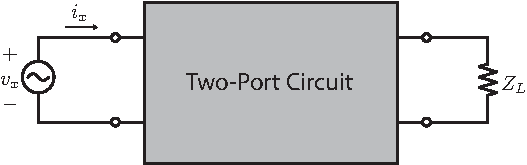
\includegraphics[width=.5\columnwidth]{2port_zin_vx} &
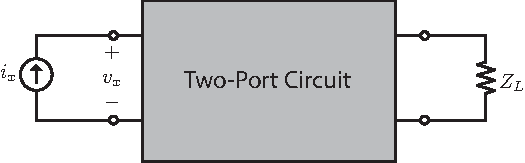
\includegraphics[width=.5\columnwidth]{2port_zin_ix} \\
(a) & (b) \\
\end{tabular}
\end{center}
\caption{To calculate the input impedance of a two-port, we apply a test (a) voltage or (b) current source and measure the current/voltage.  By convention, we leave the output resistance connected to the load.}
\label{fig:2port_zin_vx}
\end{figure}
%%%%%%%%%%%%%%%%%%%%%%%%%%%%%%%%%%%%%%%%%%%%
%             SUBSECTION 12.2.4            %
%%%%%%%%%%%%%%%%%%%%%%%%%%%%%%%%%%%%%%%%%%%%
\subsection{Output Impedance $Z_{out}$}
We measure the output impedance in the same manner as the input impedance.  Again, if the amplifier were truly unilateral, connecting a source at the output would not affect the input port, but due to parasitic leakage (say through capacitance), there is a small influence.  By convention, the \textit{input} port is terminated with the \textit{source} resistance, and the output port is measured, as shown in Fig.~\ref{fig:2port_zout_vx}.
For example, we can excite with a test voltage (current) source, and then measure the output current (voltage):
\begin{equation}
	{Z_{out}} = {\left. {\frac{{{v_x}}}{{{i_x}}}} \right|_{\scriptstyle{Z_L}\,\text{removed},\hfill\atop
	\scriptstyle{Z_S}\,\text{attached}\hfill}}
\end{equation}
%%%%%%%%%%%%%%%%%%%%%%%%%%%%%%%%%%%%%%%%%%%%
%                 FIGURE                   %
%%%%%%%%%%%%%%%%%%%%%%%%%%%%%%%%%%%%%%%%%%%%
\begin{figure}[tb]
\begin{center}
\begin{tabular}{cc}
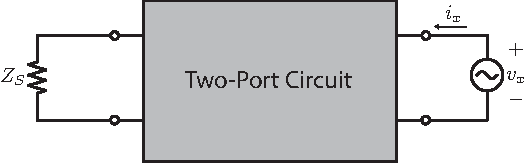
\includegraphics[width=.5\columnwidth]{2port_zout_vx} &
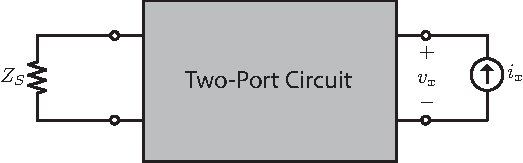
\includegraphics[width=.5\columnwidth]{2port_zout_ix} \\
(a) & (b) \\
\end{tabular}
\end{center}
\caption{To calculate the output impedance of a two-port, we apply a test (a) voltage or (b) current source and measure the current/voltage.  By convention, we leave the source resistance connected to the input.}
\label{fig:2port_zout_vx}
\end{figure}
%%%%%%%%%%%%%%%%%%%%%%%%%%%%%%%%%%%%%%%%%%%%%%%%%%%%%%%%%%%%%%%%%%%%%%%%%%%%%%%%%%%%%%%%
%%%%%%%%%%%%%%%%%%%%%%%%%%%%%%%%%%%%%%%%%%%%%%%%%%%%%%%%%%%%%%%%%%%%%%%%%%%%%%%%%%%%%%%%
%                                   SECTION 12.3                                       %
%%%%%%%%%%%%%%%%%%%%%%%%%%%%%%%%%%%%%%%%%%%%%%%%%%%%%%%%%%%%%%%%%%%%%%%%%%%%%%%%%%%%%%%%
%%%%%%%%%%%%%%%%%%%%%%%%%%%%%%%%%%%%%%%%%%%%%%%%%%%%%%%%%%%%%%%%%%%%%%%%%%%%%%%%%%%%%%%%
\section{Single-Stage MOS Amplifier Family}
Since a transistor is a three-terminal device (ignoring the body terminal of a MOSFET), and an amplifier is a four terminal two-port, constructing an amplifier out of a transistor requires one terminal to be in ``common" with both ports.  This leads to the family of amplifiers shown in Fig.~\ref{fig:ampchart}, the Common Source (CS) amplifier already studied extensively in the previous chapters on small-signal modeling, the common-gate (CG) amplifier, and the Common Drain (CD) amplifier.  The BJT equivalents are the Common Emitter (CE), Common Base (CB), and the Common Collector (CC).  In this chapter we will focus on the MOS amplifiers and with relatively small changes we can apply our knowledge to BJT amplifiers as well.  While this is true of the small-signal models, the large-signal behavior, such as the operating point, requires a very different approach.
%%%%%%%%%%%%%%%%%%%%%%%%%%%%%%%%%%%%%%%%%%%%
%                 FIGURE                   %
%%%%%%%%%%%%%%%%%%%%%%%%%%%%%%%%%%%%%%%%%%%%
\begin{figure}[tb]
\begin{center}
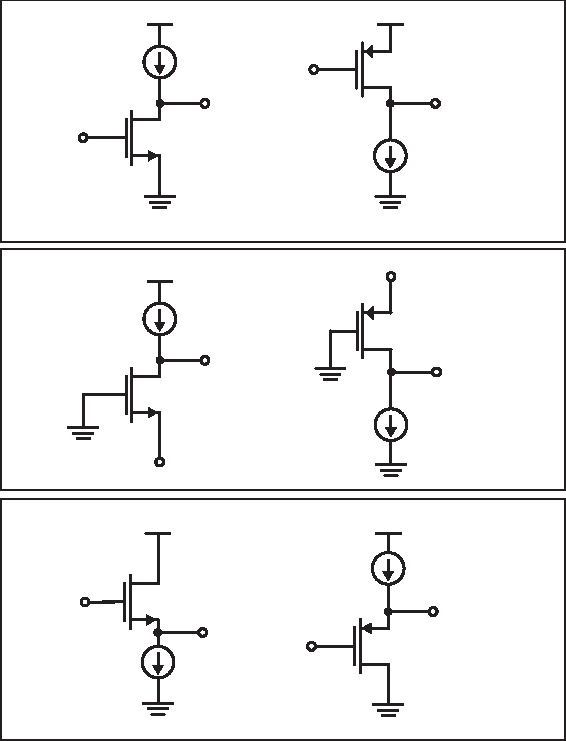
\includegraphics[scale=.75]{ampchart}
\end{center}
\caption{Family of NMOS and PMOS single-stage amplifiers.  Listing from the top, the Common Source, Common-Gate, and Common Drain Amplifiers.  As shown, each is biased with an ideal current source while in practice we use transistor based current mirrors (see Ch.~\ref{ch:mirrors}) or resistors to bias the amplifiers.}
\label{fig:ampchart}
\end{figure}
%%%%%%%%%%%%%%%%%%%%%%%%%%%%%%%%%%%%%%%%%%%%
%             SUBSECTION 12.3.1            %
%%%%%%%%%%%%%%%%%%%%%%%%%%%%%%%%%%%%%%%%%%%%
\subsection{Isolating the Bias Points}
%%%%%%%%%%%%%%%%%%%%%%%%%%%%%%%%%%%%%%%%%%%%
%                 FIGURE                   %
%%%%%%%%%%%%%%%%%%%%%%%%%%%%%%%%%%%%%%%%%%%%
\begin{figure}[tb]
\begin{center}
\begin{tabular}{cc}
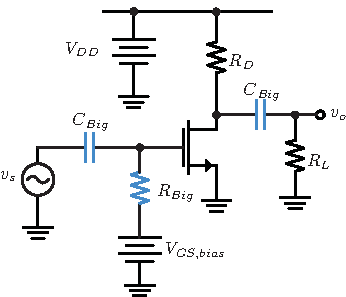
\includegraphics[width=.4\columnwidth]{csamp_bias} &
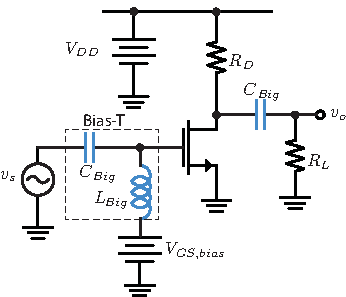
\includegraphics[width=.4\columnwidth]{csamp_biasT} \\
(a) & (b) \\
\end{tabular}
\end{center}
\caption{(a) AC coupling capacitors are large (ideally infinite) and act like batteries, allowing different points in a circuit to be biased to different DC values, effectively blocking DC but allowing AC signals to flow.  A large resistor is used to ``block" the AC signals without loading the circuit.  (b) Large biasing inductors, sometimes called ``chokes" are used to apply a DC voltage to a node while acting like an open-circuit at AC frequencies.  A combination of an inductor and capacitor forms a bias-T.}
\label{fig:ac_couple}
\end{figure}

When hooking up a source or load to an amplifier, it's easy to change the DC operating point.  One solution, adopted with discrete amplifiers, is to use a large ``AC coupling" capacitors at the input and/or output to isolate the load, as shown in Fig.~\ref{fig:ac_couple}a. Think of a very large capacitors as a battery. At AC frequencies, it acts like a short circuit.  One way to emphasize these capacitors as very large is to label them with $C_\infty$. This indicates that they are ideally infinitely large capacitors so that they act as short circuits for any non-zero frequency.  Often we also need to block AC signals from getting shorted out by bias voltages.  One solution adopted (shown in the figure) is a large resistor.  The resistors are made large enough to avoid loading the amplifier.
%%%%%%%%%%%%%%%%%%%%%%%%%%%%%%%%%%%%%%%%%%%%
%              SUB-SUBSECTION              %
%%%%%%%%%%%%%%%%%%%%%%%%%%%%%%%%%%%%%%%%%%%%
\subsubsection{``Chokes"}
In place of large resistors, infinitely large inductors, or ``chokes" as they are sometimes called, are also convenient, as they work at DC but at any non-zero frequency they are essentially open circuits.  Chokes are also used to isolate the DC supply or reference voltages of sensitive circuits from the rest of the (noisy) system, as shown in Fig.~\ref{fig:ac_couple}b.
%%%%%%%%%%%%%%%%%%%%%%%%%%%%%%%%%%%%%%%%%%%%
%             SUBSECTION 12.3.2            %
%%%%%%%%%%%%%%%%%%%%%%%%%%%%%%%%%%%%%%%%%%%%
\subsection{DC Coupled vs AC Coupled Amplifiers}
%%%%%%%%%%%%%%%%%%%%%%%%%%%%%%%%%%%%%%%%%%%%
%                 FIGURE                   %
%%%%%%%%%%%%%%%%%%%%%%%%%%%%%%%%%%%%%%%%%%%%
\begin{figure}[tb]
\begin{center}
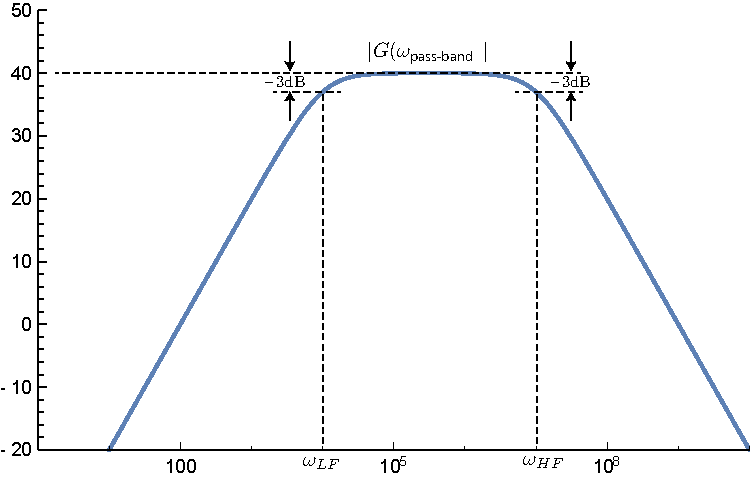
\includegraphics[width=.6\columnwidth]{amp_bandpass}
\end{center}
\caption{Definition of the ``mid-band" or ``pass-band" of an amplifier occurs at AC frequencies where large capacitors act like shorts (and large inductors are open).}
\label{fig:cgamp_is}
\end{figure}

AC coupled amplifiers have no gain at DC because the capacitors are ``open" at very low frequencies, or alternatively the chokes short out the signal at DC.  With reference to Fig.~\ref{fig:midband}, the midband is defined as the region where the gain is approximately flat, before rolling off due to high frequency effects, and after recovering from the effect of large capacitors. The general rule is to replace large capacitors with shorts, and small capacitors (transistor parasitics for example) as opens when finding the \emph{midband gain}. 
%%%%%%%%%%%%%%%%%%%%%%%%%%%%%%%%%%%%%%%%%%%%
%             SUBSECTION 12.3.3            %
%%%%%%%%%%%%%%%%%%%%%%%%%%%%%%%%%%%%%%%%%%%%
\subsection{Common-Gate (CG) Amplifier}
%%%%%%%%%%%%%%%%%%%%%%%%%%%%%%%%%%%%%%%%%%%%
%                 FIGURE                   %
%%%%%%%%%%%%%%%%%%%%%%%%%%%%%%%%%%%%%%%%%%%%
\begin{figure}[tb]
\begin{center}
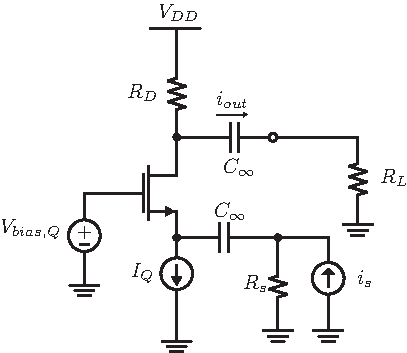
\includegraphics[scale=1]{cgamp_is}
\end{center}
\caption{The schematic of a common-gate amplifier driven by a source $i_s$ with source resistance $R_s$.  Capacitors are used to block the source/load DC levels from the amplifier, which is biased through $I_Q$ and $V_{bias,Q}$.}
\label{fig:cgamp_is}
\end{figure}
 
The common-gate amplifier is shown in Fig.~\ref{fig:cgamp_is}.  The current source $I_Q$ and voltage source $V_{bias,Q}$ are DC supplies used to bias the amplifier.  The signal $i_s$ and resistor $R_s$ form the AC signal source, and they are isolated by a large capacitor.  Likewise, the load $R_L$ is isolated by another capacitor.  Notice that without these capacitors, the DC points at the source and drain would shift.  The DC operating point of the amplifier is simply given by
\begin{equation}
	{I_Q} = {I_{DS}}
\end{equation}
Since $V_{bias,Q}$ does not appear in the equation, you may be wondering why we don't simply ground the gate, as the circuit functionality is unaffected.  For an ideal current source, operating the gate at ground would bring the source node to a negative voltage.  We will learn in the next chapter that real current sources will cease to function under such conditions, and the gate bias voltage is there to provide some ``headroom" to the current source $I_Q$.
%%%%%%%%%%%%%%%%%%%%%%%%%%%%%%%%%%%%%%%%%%%%
%             SUBSECTION 12.3.4            %
%%%%%%%%%%%%%%%%%%%%%%%%%%%%%%%%%%%%%%%%%%%%
\subsection{Common-Gate AC Model}
%%%%%%%%%%%%%%%%%%%%%%%%%%%%%%%%%%%%%%%%%%%%
%                 FIGURE                   %
%%%%%%%%%%%%%%%%%%%%%%%%%%%%%%%%%%%%%%%%%%%%
\begin{figure}[tb]
\begin{center}
\begin{tabular}{cc}
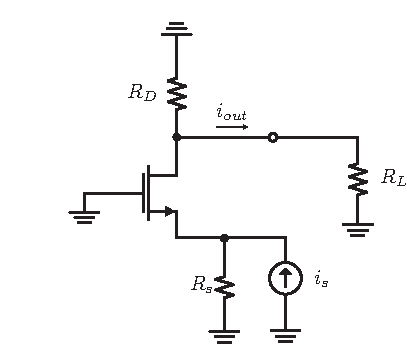
\includegraphics[scale=.9]{cgamp_is_ac} &
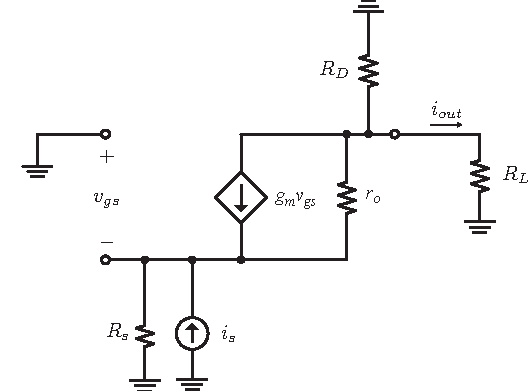
\includegraphics[scale=.9]{cgamp_is_ac_ss} \\
(a) & (b) \\
\end{tabular}
\end{center}
\caption{(a) The AC equivalent schematic of the common-gate amplifier.  (b) The small-signal equivalent circuit of the common-gate amplifier.}
\label{fig:cgamp_is_ac}
\end{figure}

The AC equivalent circuit model is shown in Fig.~\ref{fig:cgamp_is_ac}a, which is obtained from Fig.~\ref{fig:cgamp_is} by simply shorting out all the DC sources.  To analyze the circuit, we can replace the transistor with its hybrid-pi equivalent circuit model, shown in Fig.~\ref{fig:cgamp_is_ac}b.
%%%%%%%%%%%%%%%%%%%%%%%%%%%%%%%%%%%%%%%%%%%%
%             SUBSECTION 12.3.5            %
%%%%%%%%%%%%%%%%%%%%%%%%%%%%%%%%%%%%%%%%%%%%
\subsection{CG as a Current Amplifier: Find $A_{i}$}
%%%%%%%%%%%%%%%%%%%%%%%%%%%%%%%%%%%%%%%%%%%%
%                 FIGURE                   %
%%%%%%%%%%%%%%%%%%%%%%%%%%%%%%%%%%%%%%%%%%%%
\begin{figure}[tb]
\begin{center}
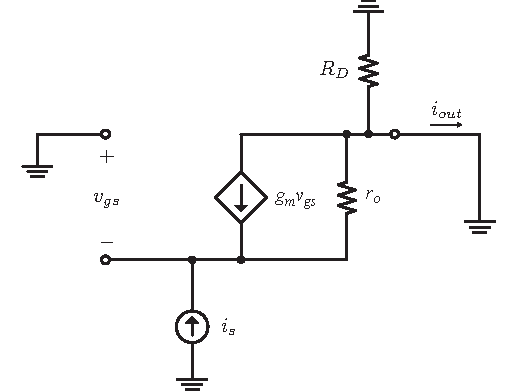
\includegraphics[scale=.9]{cgamp_is_ac_ss_short}
\end{center}
\caption{To find the intrinsic current gain of a common-gate amplifier, we short the output and drive the input with an ideal current source.  The current gain is the current flowing out $i_{out}$ divided by $i_s$.}
\label{fig:cgamp_is_ac_ss_short}
\end{figure}

We will first analyze the circuit as a current amplifier.  To find the current gain of a current amplifier, we should short-circuit the output and observe the output current (flowing into the short) when driven by an ideal current source.  This means we drive it with a current source with zero source conductance, as shown in Fig.~\ref{fig:cgamp_is_ac_ss_rout}.  Notice that the output current is the drain.  Also notice that the source current must flow through the output because that's the only path for the current to return:
\begin{equation}
	{i_{out}} = {i_d} =  - {i_s}
\end{equation}
From these observations, it's obvious that the current gain is given by:
\begin{equation}
	{A_i} =  - 1
\end{equation}
%%%%%%%%%%%%%%%%%%%%%%%%%%%%%%%%%%%%%%%%%%%%
%             SUBSECTION 12.3.6            %
%%%%%%%%%%%%%%%%%%%%%%%%%%%%%%%%%%%%%%%%%%%%
\subsection{CG Input Resistance}
%%%%%%%%%%%%%%%%%%%%%%%%%%%%%%%%%%%%%%%%%%%%
%                 FIGURE                   %
%%%%%%%%%%%%%%%%%%%%%%%%%%%%%%%%%%%%%%%%%%%%
\begin{figure}[tb]
\begin{center}
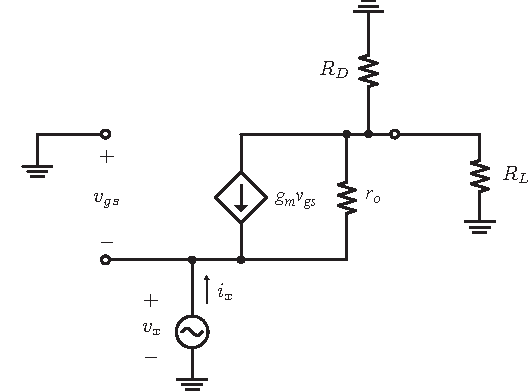
\includegraphics[scale=.9]{cgamp_is_ac_ss_zin}
\end{center}
\caption{To determine the input impedance of a common-gate amplifier, we drive the input with a test source $v_x$ and measure the current $i_x$ flowing into the amplifier.  By convention, we leave the load resistance connected at the output.}
\label{fig:cgamp_is_ac_ss_zin}
\end{figure}

Next we calculate the input impedance of the CG amplifier.  By convention, we leave the load resistance connected at the output and we apply a test source.  We can use a test voltage $v_x$ or a current.  In Fig.~\ref{fig:cgamp_is_ac_ss_zin}, we apply a test voltage and observe the current $i_x$.  The test current splits between the transistor $r_o$ and the $g_m$ generator:
\begin{equation}
	{i_x} =  - {g_m}{v_{gs}} + \left( {\frac{{{v_x} - {v_{out}}}}{{{r_o}}}} \right) \label{eq:cg_input}
\end{equation}
At the output of the amplifier, the current flows into the load resistor $R_L$ in parallel with $R_D$:
\begin{equation}
	{v_{out}} =  - {i_d}({R_D}||{R_L}) = {i_x}({R_D}||{R_L})
\end{equation}
Also notice that the voltage $v_{gs}$ is in fact just the negative of the test source.  With these observations, we substitute into Eq.~\ref{eq:cg_input} to obtain:
\begin{equation}
	{i_x} = {g_m}{v_x} + \left( {\frac{{{v_x} - \left( {{R_D}||{R_L}} \right){i_x}}}{{{r_o}}}} \right)
\end{equation}
Which results in the input conductance taking the form:
\begin{equation}
	G_{in} = \frac{1}{{{R_{in}}}} = \frac{{{i_t}}}{{{v_x}}} = \frac{{{g_m} + \frac{1}{{{r_o}}}}}{{1 + \frac{{{R_D}||{R_L}}}{{{r_o}}}}} \label{eq:cg_zin2}
\end{equation}
Notice that the input impedance depends on the load, an undesirable result.  But as we shall see, the dependence on the load is rather weak.  Let's make some approximations to simplify the results.  First of all, a good transistor has good intrinsic voltage gain $A_0$: 
\begin{equation}
	A_0 = g_m r_o \gg 1
\end{equation}
If we factor $g_m$ out from Eq.~\ref{eq:cg_zin2}
\begin{equation}
	G_{in} = g_m \frac{{1 + \frac{1}{{{g_m r_o}}}}}{{1 + \frac{{{R_D}||{R_L}}}{{{r_o}}}}}
\end{equation}
Next let's assume that $r_o \gg R_D||R_L$, which allows us to simplify to
\begin{equation}
	{R_{in}} = \frac{1}{{{g_m}}}
\end{equation}
Does this result make sense?  After some careful deliberation, it is actually somewhat intuitive, at least in the limit that we have obtained in the approximation.  To see this ignore the output node and assume it's grounded (drain is grounded). Modulating the source voltage modulates the $v_{sg}$ of the transistor, which causes the current to increase by $-g_m v_{sg}$, resulting in an input conductance of $g_m$.  In the absence of $R_D$ and $R_L$, the only correction to this would be to account for $r_o$, which simply is in parallel, so the input conductance would be $g_m + 1/r_o$.  But the presence of the load $R_D || R_L$ complicates things a bit.  In practice we usually satisfy the condition that $R_D || R_L \ll r_o$, so the simple result is enough. 
%%%%%%%%%%%%%%%%%%%%%%%%%%%%%%%%%%%%%%%%%%%%
%             SUBSECTION 12.3.7            %
%%%%%%%%%%%%%%%%%%%%%%%%%%%%%%%%%%%%%%%%%%%%
\subsection{CG Output Resistance}
%%%%%%%%%%%%%%%%%%%%%%%%%%%%%%%%%%%%%%%%%%%%
%                 FIGURE                   %
%%%%%%%%%%%%%%%%%%%%%%%%%%%%%%%%%%%%%%%%%%%%
\begin{figure}[tb]
\begin{center}
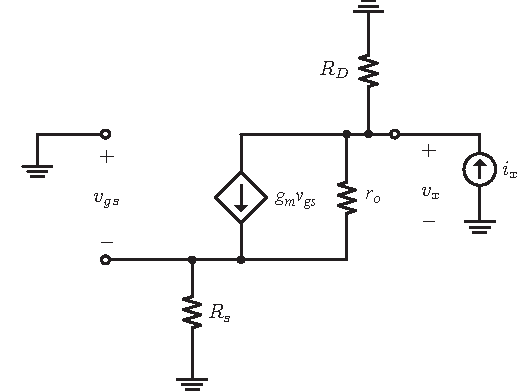
\includegraphics[scale=.9]{cgamp_is_ac_ss_rout}
\end{center}
\caption{To determine the output impedance of a common-gate amplifier, we drive the output with a test source $i_x$ and measure the voltage $v_x$.  By convention, we leave the source resistance connected at the input.}
\label{fig:cgamp_is_ac_ss_rout}
\end{figure}

To find the CG amplifier output impedance, let's connect a test current source $i_x$ at the output and observe the voltage $v_x$, as shown in Fig.~\ref{fig:cgamp_is_ac_ss_rout}.  Write KCL at the input of the amplifier:
\begin{equation}
	\frac{{{v_s}}}{{{R_S}}} - {g_m}{v_{gs}} + \frac{{{v_s} - {v_x}}}{{{r_o}}} = 0
\end{equation}
Let's make a simplifying step and eliminate $R_D$ for a moment, since it will simply load the output in an obvious way (in parallel with the transistor effective output impedance).  In this case, notice that the voltage at the source $v_s = i_x R_S$, since $i_x$ would flow entirely through $R_S$ (without $R_D$), and also $v_{gs} = -v_s$, so the above equation can be simplified to:
\begin{equation}
	{v_s}\left( {\frac{1}{{{R_S}}} + {g_m} + \frac{1}{{{r_o}}}} \right) = \frac{{{v_x}}}{{{r_o}}}
\end{equation}
This expression implies that the effective output impedance looking into the drain of the amplifier, in the presence of $R_S$, is boosted to
\begin{equation}
	R_{out,\text{no $R_D$}} =  {{R_S}\left( {\frac{{{r_o}}}{{{R_S}}} + {g_m}{r_o} + 1} \right)} 
\end{equation}
Bringing back $R_D$:
\begin{equation}
	{R_{out}} = {R_D}||\left( {{r_o} + {g_m}{r_o}{R_S} + {R_S}} \right) 
\end{equation}
This is a very interesting result, and not so obvious.  Adding a resistor $R_S$ in series with the transistor on the drain side would simply increase the resistance to $r_o + R_S$.  On the other hand, adding such a resistor on the source side increased the output impedance by a factor of $1 + g_m R_S$, potentially a large factor.  To understand why this happens, we must use feedback theory, something that you will learn in the future.

The exact result is complicated, and a simpler version is easier to remember and nearly as accurate:
\begin{equation} 
	{R_{out}} \cong {R_D}||[{r_o} + {g_m}{r_o}{R_S} + {R_S}] \approx R_D || (1 + g_m R_S) r_o
\end{equation}
And even simpler version can be obtained by assuming the source resistance is less than $r_o$:
\begin{equation} 
{R_{out}} \approx {R_D}||[{r_o} + {g_m}{r_o}{R_S}] = {R_D}||[{r_o}(1 + {g_m}{R_S})]
\end{equation}
%%%%%%%%%%%%%%%%%%%%%%%%%%%%%%%%%%%%%%%%%%%%
%             SUBSECTION 12.3.8            %
%%%%%%%%%%%%%%%%%%%%%%%%%%%%%%%%%%%%%%%%%%%%
\subsection{CG Two-Port Model}
%%%%%%%%%%%%%%%%%%%%%%%%%%%%%%%%%%%%%%%%%%%%
%                 FIGURE                   %
%%%%%%%%%%%%%%%%%%%%%%%%%%%%%%%%%%%%%%%%%%%%
\begin{figure}[tb]
\begin{center}
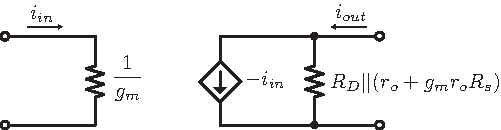
\includegraphics[scale=.9]{cg_model}
\end{center}
\caption{A two-port model for the CG amplifier is a current buffer with input impedance $1/g_m$ and otuput impedance as shown.  }
\label{fig:cg_model}
\end{figure}

We can summarize everything we've learned about the CG amplifier thus far by building an equivalent model of the CG amplifier, shown in Fig.~\ref{fig:cg_model}.  This is a current amplifier model with a current gain of unity, which means it's a ``Current Buffer".  A current buffer needs to meet three requirements:  (1) It must have a current gain of unity; (2) it should present a low input impedance;  (3) it should present a high output impedance.  Under these three conditions, the output current into a load is a faithful reproduction of the input.  It is extremely important to understand the role of low input impedance and high output impedance in this functionality.  A CS amplifier is not a good current buffer because it fails the first two criteria.  It's not even a good current amplifier because it does not satisfy the second criteria at low frequencies.  At sufficiently high frequencies, though, we can think of it as a current amplifier.   If this idea of a ``Current Buffer" is not making sense, take some time and calculate the current gain of a two-port Current Amplifier under arbitrary load and source impedance.  Then find the conditions for the externally observed current gain to match the internal current gain of the amplifier.
%%%%%%%%%%%%%%%%%%%%%%%%%%%%%%%%%%%%%%%%%%%%
%             SUBSECTION 12.3.9            %
%%%%%%%%%%%%%%%%%%%%%%%%%%%%%%%%%%%%%%%%%%%%
\subsection{Common-Gate as a ``Voltage Amplifier"}
%%%%%%%%%%%%%%%%%%%%%%%%%%%%%%%%%%%%%%%%%%%%
%                 FIGURE                   %
%%%%%%%%%%%%%%%%%%%%%%%%%%%%%%%%%%%%%%%%%%%%
\begin{figure}[tb]
\begin{center}
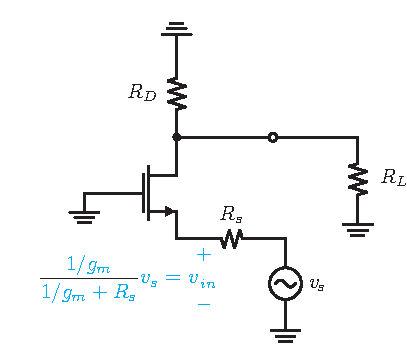
\includegraphics[scale=1]{cgamp_vs_ac}
\end{center}
\caption{When the common-gate amplifier is voltage driven, the input voltage source is divided between its source resistance and the input of the amplifier, reducing the gain.}
\label{fig:cg_v_amp}
\end{figure}

If we voltage drive the CG amplifier, as shown in Fig.~\ref{fig:cg_v_amp}, with source resistance $R_S = 0\Omega$, then the $g_m$ is the same as a CS, and the gain is also just as good as a CS amplifier (with opposite phase):
\begin{equation}
	v_{gs} = -v_s 
\end{equation}
\begin{equation}
	v_{o} = - i_d R_L||R_D =  - (-g_m v_s) R_L||R_D 
\end{equation}
\begin{equation}
	A_v = g_m R_L||R_D
\end{equation}
But if we have source resistance, then the low input impedance causes a voltage divider effect:
\begin{equation}
	v_{gs} = -v_s \frac{Z_{in}}{Z_{in} + R_s} = -v_s \frac{1/g_m}{1/g_m + R_s} = - \frac{v_s}{1 + g_m R_s}
\end{equation}
This results a lower transconductance:
\begin{equation}
	v_{o} = - i_d R_L||R_D =  - \frac{-v_s g_m }{1 + g_m R_s} R_L||R_D 
\end{equation}
And consequently a lower voltage gain: 
\begin{equation}
	A_v = \frac{g_m }{1 + g_m R_s} R_L||R_D
\end{equation}
This analysis is important because it shows that a CG amplifier can be interpreted in different ways.  It's not only a current buffer, it can provide voltage gain and be viewed as a voltage amplifier, it's just that it's input impedance is low and so it will likely load the source.  In some applications, such as RF amplifiers, this is desirable because for power matching we desire the load and the source impedance to match (to extract the maximum power from the source), and the CG low input impedance is a convenient match to $75\Omega$ or $50\Omega$ transmission-line impedances.  The other benefit of the CG amplifier as a voltage amplifier, compared to the CS amplifier in particular, is that it has positive gain, as opposed to the inverting amplification of the CS stage.  In some applications, we need positive gain, or we want to combine positive gain with negative gain, for example in a differential amplifier, and so the CG amplifier will be useful.
%%%%%%%%%%%%%%%%%%%%%%%%%%%%%%%%%%%%%%%%%%%%
%                 FIGURE                   %
%%%%%%%%%%%%%%%%%%%%%%%%%%%%%%%%%%%%%%%%%%%%
\begin{figure}[tb]
\begin{center}
\begin{tabular}{cc}
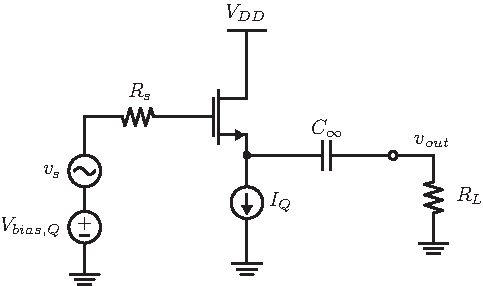
\includegraphics[scale=.9]{cd_amp_dc} &
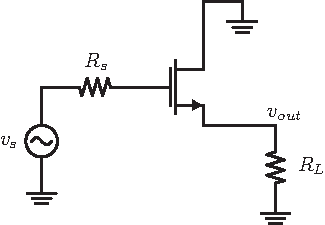
\includegraphics[scale=.9]{cd_amp_ac} \\
(a) & (b) \\
\end{tabular}
\end{center}
\caption{(a) The Common Drain (CD) amplifier full schematic.  (b) AC equivalent circuit of CD amplifier.}
\label{fig:cd_amp_dc_ac}
\end{figure}
%%%%%%%%%%%%%%%%%%%%%%%%%%%%%%%%%%%%%%%%%%%%%%%%%%%%%%%%%%%%%%%%%%%%%%%%%%%%%%%%%%%%%%%%
%%%%%%%%%%%%%%%%%%%%%%%%%%%%%%%%%%%%%%%%%%%%%%%%%%%%%%%%%%%%%%%%%%%%%%%%%%%%%%%%%%%%%%%%
%                                   SECTION 12.4                                       %
%%%%%%%%%%%%%%%%%%%%%%%%%%%%%%%%%%%%%%%%%%%%%%%%%%%%%%%%%%%%%%%%%%%%%%%%%%%%%%%%%%%%%%%%
%%%%%%%%%%%%%%%%%%%%%%%%%%%%%%%%%%%%%%%%%%%%%%%%%%%%%%%%%%%%%%%%%%%%%%%%%%%%%%%%%%%%%%%%
\section{Common Drain Amplifier}
The full schematic of the Common Drain amplifier is shown in Fig.~\ref{fig:cd_amp_dc_ac}a.  The ``common" terminal is obviously the drain, but unlike the CG and CS amplifiers, it's not grounded, but connected to a DC supply.  This is because we need to connect the drain to a higher potential than the gate/source in order to bias the transistor in saturation.  As far as AC signals are concerned, though, the drain voltage is DC and therefore AC grounded, as shown in Fig.~\ref{fig:cd_amp_dc_ac}b.
%%%%%%%%%%%%%%%%%%%%%%%%%%%%%%%%%%%%%%%%%%%%
%             SUBSECTION 12.4.1            %
%%%%%%%%%%%%%%%%%%%%%%%%%%%%%%%%%%%%%%%%%%%%
\subsection{CD DC Operating Point}
The CD amplifier is usually biased with a constant current $I_Q$ as shown.  The load is AC coupled and so the transistor $I_{DS}$ flows into $I_Q$:
\begin{equation}
	I_Q = {I_{DS}} = \mu {C_{ox}}\frac{W}{L}\frac{1}{2}{({V_{GS}} - {V_T})^2}	
\end{equation}
In theory, the gate voltage could be at any DC bias point, but in practice we know that the current $I_Q$ dictates a positive $V_{GS}$:
\begin{equation}
	{V_{GS}} = {V_T} + \sqrt {\frac{{2{I_{Q}}}}{{\mu {C_{ox}}\frac{W}{L}}}} 
\end{equation}
To give the current source $I_Q$ some headroom (DC voltage), we need to bias the gate of the transistor at a correspondingly higher voltage.  For now let's call that $V_{bias,Q}$ similar to the CG amplifier.
%%%%%%%%%%%%%%%%%%%%%%%%%%%%%%%%%%%%%%%%%%%%
%             SUBSECTION 12.4.2            %
%%%%%%%%%%%%%%%%%%%%%%%%%%%%%%%%%%%%%%%%%%%%
\subsection{CD Voltage Gain}
%%%%%%%%%%%%%%%%%%%%%%%%%%%%%%%%%%%%%%%%%%%%
%                 FIGURE                   %
%%%%%%%%%%%%%%%%%%%%%%%%%%%%%%%%%%%%%%%%%%%%
\begin{figure}[tb]
\begin{center}
\begin{tabular}{cc}
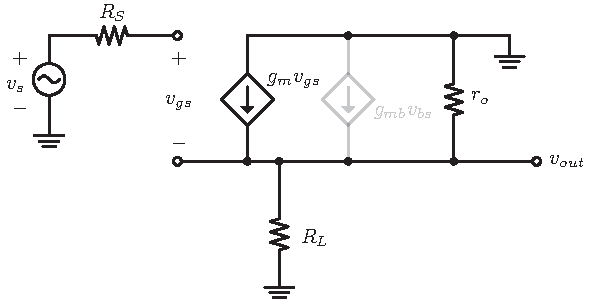
\includegraphics[scale=.75]{cd_amp_ss_av2} &
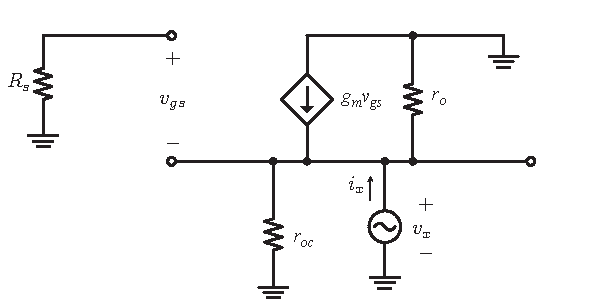
\includegraphics[scale=.75]{cd_amp_ss_rout} \\
(a) & (b) \\
\end{tabular}
\end{center}
\caption{(a) Common Drain amplifier small-signal equivalent circuit.  (b)  Small-signal circuit schematic for calculation of output impedance.}
\label{fig:cd_amp_ss_av2}
\end{figure}

To find the voltage gain of the CD amplifier, we apply an AC source to the gate and observe the output voltage at the source, as shown in Fig.~\ref{fig:cd_amp_ss_av2}.  In the small-signal model, we have grayed out the back-gate generator $g_{mb}$, which would be the case if we short the source to the body of the transistor.  We will handle the situation of the grounded body later. Let's write KCL at the output node:
\begin{equation}
	\frac{{{v_{out}}}}{{{R_L}||{r_o}}} = {g_m}{v_{gs}}
\end{equation}
Since the input and output are just separated by $v_{gs}$, or $v_{gs} = v_{s} - v_{out}$, we have
\begin{equation}
	\frac{{{v_{out}}}}{{{R_L}||{r_o}}} = {g_m}\left( {{v_{s}} - {v_{out}}} \right)
\end{equation}
Collecting common factors:
\begin{equation}
	\left( {\frac{1}{{{R_L}||{r_o}}} + {g_m}} \right){v_{out}} = {g_m}{v_{s}}
\end{equation}
This last equation leads us to the voltage gain:
\begin{equation}
	\frac{{{v_{out}}}}{{{v_{s}}}} = \frac{{{g_m}}}{{\frac{1}{{{R_L}||{r_o}}} + {g_m}}}
\end{equation}
Assuming that $r_o \gg R_L$, we have
\begin{equation}
	\frac{{{v_{out}}}}{{{v_{s}}}} \approx \frac{{{g_m}}}{{1/{R_L} + {g_m}}} \approx 1
\end{equation}
This final result leads to another name for this amplifier, namely the ``Source Follower," since the source voltage closely tracks the gate voltage.  In other words, this is a voltage amplifier with unity gain, or a voltage buffer.

To be a voltage buffer, though, also requires high input impedance and low output impedance.  Obviously the input impedance is large, especially at low frequencies, because of the insulating nature of the gate.  Let's examine the output impedance.
%%%%%%%%%%%%%%%%%%%%%%%%%%%%%%%%%%%%%%%%%%%%
%             SUBSECTION 12.4.3            %
%%%%%%%%%%%%%%%%%%%%%%%%%%%%%%%%%%%%%%%%%%%%
\subsection{CD Output Resistance}
To calculate the output impedance, refer to Fig.~\ref{fig:cd_amp_ss_av2}b.  We apply a test source $v_x$ and find the current $i_x$.  For a moment, forget about $r_o$ and $r_{oc}$, the output resistance of the transistor and the current source.  They are simply in parallel with the source and can be added later.  In that case, let's sum currents at output (source) node:
\begin{equation}{i_x} = {g_m}{v_x}\end{equation}
which leads to:
\begin{equation}
	{R_{out}} = {r_o}||{R_L}||\frac{{{v_x}}}{{{i_x}}} = {r_o}||{R_L}||\frac{1}{g_m}
\end{equation}
If $r_o || R_L$ is much larger than the inverses of the transconductance, the output impedance is given by:
\begin{equation}
	{R_{out}} \approx \frac{1}{{{g_m}}}
\end{equation}
This equation implies that a good voltage buffer needs to be biased with a large $g_m$.  Recall that the $g_m$ of a transistor is proportional to $\sqrt{I_{DS}}$, so a good voltage buffer is realized by burning sufficiently large DC current.  Indeed, the CD amplifier is often used as an output stage to drive a heavy load.  A heavy load is a small resistance, because for a fixed voltage swing it draws more power than a larger resistor.  In order to buffer a gain stage from a small load, we can add a Source Follower amplifier.  

Finally, if we put everything together, we can see that a CD amplifier, or a Source Follower, is modeled as shown in Fig.~\ref{fig:cd_amp_model}.  
%%%%%%%%%%%%%%%%%%%%%%%%%%%%%%%%%%%%%%%%%%%%
%                 FIGURE                   %
%%%%%%%%%%%%%%%%%%%%%%%%%%%%%%%%%%%%%%%%%%%%
\begin{figure}[tb]
\begin{center}
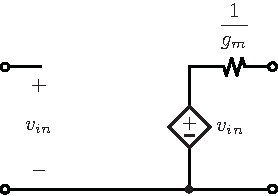
\includegraphics[scale=1]{cd_amp_model}
\end{center}
\caption{A two-port model for the CD amplifier is a voltage buffer with unity gain and output impedance $1/g_m$.}
\label{fig:cd_amp_model}
\end{figure}
%%%%%%%%%%%%%%%%%%%%%%%%%%%%%%%%%%%%%%%%%%%%%%%%%%%%%%%%%%%%%%%%%%%%%%%%%%%%%%%%%%%%%%%%
%%%%%%%%%%%%%%%%%%%%%%%%%%%%%%%%%%%%%%%%%%%%%%%%%%%%%%%%%%%%%%%%%%%%%%%%%%%%%%%%%%%%%%%%
%                                   SECTION 12.5                                       %
%%%%%%%%%%%%%%%%%%%%%%%%%%%%%%%%%%%%%%%%%%%%%%%%%%%%%%%%%%%%%%%%%%%%%%%%%%%%%%%%%%%%%%%%
%%%%%%%%%%%%%%%%%%%%%%%%%%%%%%%%%%%%%%%%%%%%%%%%%%%%%%%%%%%%%%%%%%%%%%%%%%%%%%%%%%%%%%%%
\section{Impact of Body Effect}
%%%%%%%%%%%%%%%%%%%%%%%%%%%%%%%%%%%%%%%%%%%%
%                 FIGURE                   %
%%%%%%%%%%%%%%%%%%%%%%%%%%%%%%%%%%%%%%%%%%%%
\begin{figure}[tb]
\begin{center}
\begin{tabular}{cc}
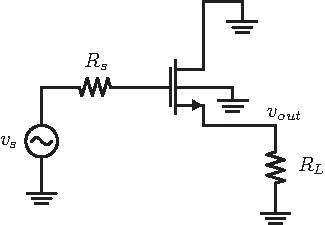
\includegraphics[scale=1]{cd_amp_ac_body} &
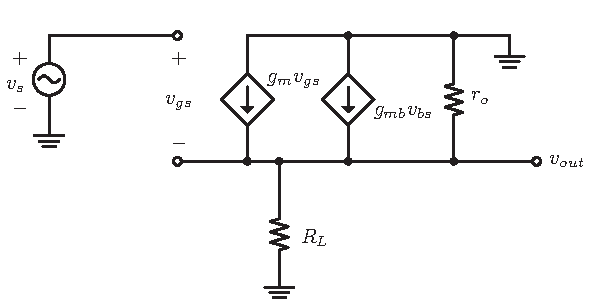
\includegraphics[scale=.8]{cd_amp_ss_av_body 2}
\end{tabular}
\end{center}
\caption{(a) The CD amplifier built with a four terminal MOSFET with a grounded body.  Note that the voltage $v_{sb}$ is not zero and therefore we must consider (b) the complete low-frequency small-signal schematic of the CD amplifier (including the back-gate effect).}
\label{fig:cd_amp_ac_body}
\end{figure}

As we noted earlier, if the source and body are not tied together, there's a back-gate effect that we need to consider.  Recall that if an NMOS transistor is fabricated in a p-type substrate, then its body connection is the substrate, which must be grounded in an IC (or tied to the lowest potential), as shown in Fig.~\ref{fig:cd_amp_ac_body}a.  It's possible to create a ``triple well" process (or a ``deep nwell" process) to accommodate placing NMOS devices in their own body wells to prevent the back-gate effect, but these process options are more expensive and increase the size of the device.  Often many NMOS devices will reside in the same substrate or pwell and so all the bodies are tied to a common (ground) node.

To calculate the gain with the back-gate effect, we return to the full four terminal small-signal schematic, redrawn in Fig.~\ref{fig:cd_amp_ac_body}b.  To find the voltage gain, we write KCL at the output node: 
\begin{equation}
	\frac{{{v_{out}}}}{{{R_L}||{r_o}}} = {g_m}{v_{gs}} + g_{mb} v_{bs} 
\end{equation}
As before, $v_{gs} = v_{s} - v_{out}$, but now we must consider that the source voltage moves with respect to the body:
\begin{equation}
	v_{bs} = 0 - v_{out} = -v_{out}
\end{equation}
Making these substitutions:
\begin{equation}
	\frac{{{v_{out}}}}{{{R_L}||{r_o}}} = {g_m}\left( {{v_{s}} - {v_{out}}}  - g_{mb} v_{out} \right)
\end{equation}
Collecting common factors:
\begin{equation}
	\left( {\frac{1}{{{R_L}||{r_o}}} + {g_m} + g_{mb} } \right){v_{out}} = {g_m}{v_{s}}
\end{equation}
This last equation leads us to the voltage gain:
\begin{equation}
	\frac{{{v_{out}}}}{{{v_{s}}}} = \frac{{{g_m}}}{{\frac{1}{{{R_L}||{r_o}}} + {g_m} + g_{mb}}}
\end{equation}
%%%%%%%%%%%%%%%%%%%%%%%%%%%%%%%%%%%%%%%%%%%%%%%%%%%%%%%%%%%%%%%%%%%%%%%%%%%%%%%%%%%%%%%%
%%%%%%%%%%%%%%%%%%%%%%%%%%%%%%%%%%%%%%%%%%%%%%%%%%%%%%%%%%%%%%%%%%%%%%%%%%%%%%%%%%%%%%%%
%                                   SECTION 12.6                                       %
%%%%%%%%%%%%%%%%%%%%%%%%%%%%%%%%%%%%%%%%%%%%%%%%%%%%%%%%%%%%%%%%%%%%%%%%%%%%%%%%%%%%%%%%
%%%%%%%%%%%%%%%%%%%%%%%%%%%%%%%%%%%%%%%%%%%%%%%%%%%%%%%%%%%%%%%%%%%%%%%%%%%%%%%%%%%%%%%%
\section{Chapter Summary: Amplifiers $\rightarrow$ $G_m$/$V$/$I$}
%%%%%%%%%%%%%%%%%%%%%%%%%%%%%%%%%%%%%%%%%%%%
%                 FIGURE                   %
%%%%%%%%%%%%%%%%%%%%%%%%%%%%%%%%%%%%%%%%%%%%
\begin{figure}[tb]
\begin{center}
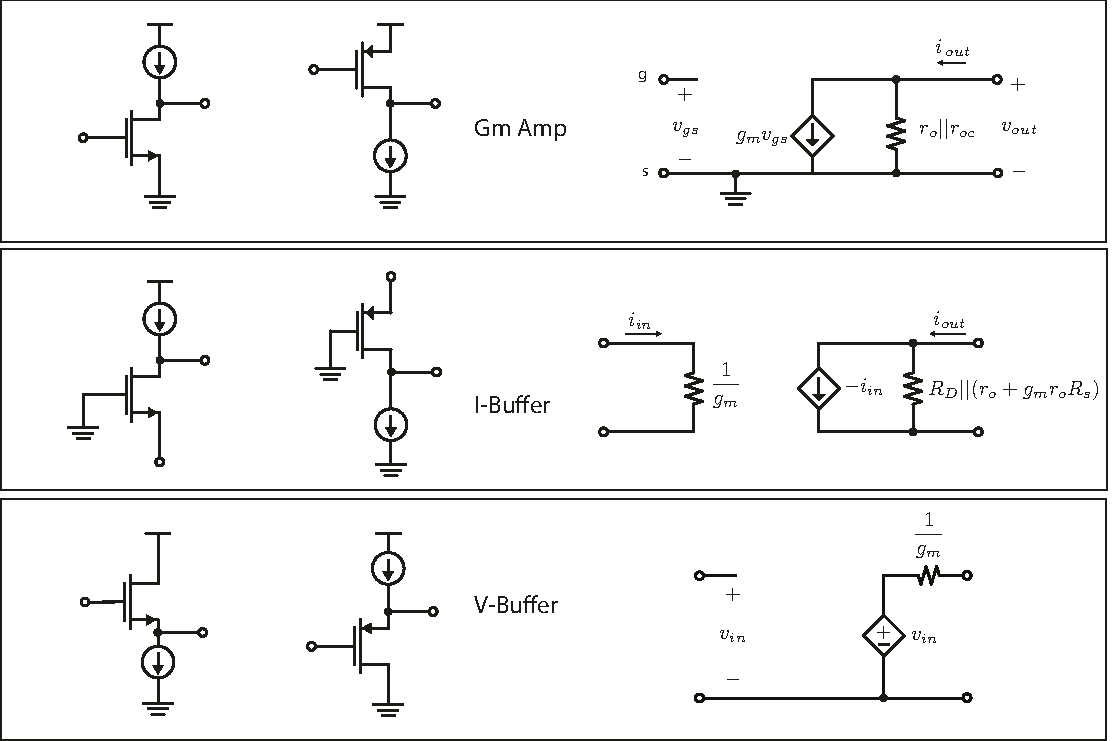
\includegraphics[width=\columnwidth]{ampchart_models}
\end{center}
\caption{The family of single-stage transistor amplifiers and the corresponding two-port models.  As you analyze more circuits, this chart will become to be imprinted in your memory.} \label{fig:ampchart_models}
\end{figure}

Let's summarize this chapter by reviewing the three possible amplifier topologies and the equivalent circuit, all shown in Fig.~\ref{fig:ampchart_models}.  In each case we model the amplifier in a certain way that best characterizes the input/output impedance of the topology.  For example, a CS amplifier has high input impedance and high output impedance, making it an ideal transconductance amplifier.  This is not to say that it cannot be designed as a (inverting) buffer, a voltage amplifier, or a current amplifier, it's just that its native impedance level lends it well to being used as a transconductance amplifier.  

The CG amplifier is likewise best seen as a current buffer, since the input and output current are nearly identical.  But CG amplifiers make great voltage amplifiers too, provided that you can drive their input impedance.  Also, their output impedance is high, and so if it's desirable to drive a low load impedance, a voltage buffer is needed.  

Finally, the CD amplifier is best viewed as a voltage buffer, providing high input impedance and low output impedance.  Its voltage gain is less than unity, but with enough bias current we can approach unity gain.  Even though the voltage gain is always less than one, it can provide \emph{power gain} by driving a load with power without requiring much input power.
